\documentclass[12pt]{article}
\usepackage{amsmath}
\usepackage{fullpage}
\usepackage{enumerate}
\usepackage{graphicx}
\title{Robust Fiducial Marker Tracking}
\author{Joe Degol, Jason Rock, Kevin Shih}

\begin{document}
\maketitle

\section{Introduction}
Fiducial marking is [rough description of fiducial markers and why they matter].

In this project, we tackle the problem of tightly tracking a fiducial marker through a series of frames. Unlike common tracking problems such as face tracking, we require that the tracker tightly follow the four corners of a fiducial marker through various viewpoint changes. 

\section{Approach}
Because the fiducial detecting can be efficiently run in real time, we opt to use it when it is available. However, because its parameters are set to cut off at very high precisions to avoid false positives, tag detections are often missed in frames where there is too much motion blur or the size of the tag is too small due to distance and/or angle.

Our overall approach is as follows:
\begin{enumerate}
\item Extract tag detections using fiducial marker detection code
\item Track interest points across image sequences using KLT
\item Smooth over detection gaps with Extended Kalman Filtering(EKF)
\item Compute homographic projection on tracked feature points within EKF proposed area
\item Apply projection to bounding quadrilateral from previous frame to determine new 4-corner coordinates
\end{enumerate}

\subsection{Detecting Fiducial Markers}
We used April Tags [citation here] for our choice of fiducial marker. We ran the provided detection code over each frame using default parameters and recorded the 4 corners and center coordinates.
\subsection{Tracking Interest Points with KLT}

\subsection{Kalman Filtering}
Fiducial marker detections are prone to occassional loss and rather expensive to run for every frame.  It would be advantageous to be able to recover from loss and reduce the number of frames which require detection.  This problem lends itself well to an Extended Kalman Filter over the location and size of the fiducial marker.  We use a constant velocity model of the system dynamics, estimating the location and velocity for the three terms.  
\begin{align}
x_k &= \left[ \begin{array}{cccccc} 
1 & 0 & 0 & d & 0 & 0 \\
0 & 1 & 0 & 0 & d & 0 \\
0 & 0 & 1 & 0 & 0 & d \\
0 & 0 & 0 & 1 & 0 & 0\\
0 & 0 & 0 & 0 & 1 & 0\\
0 & 0 & 0 & 0 & 0 & 1
\end{array}\right] x_{k-1} + w_{k-1}\\
z_k &= \left[ \begin{array}{cccccc}
1 & 0 & 0 & 0 & 0 & 0\\
0 & 1 & 0 & 0 & 0 & 0\\
0 & 0 & 1 & 0 & 0 & 0\end{array}\right] x_k + v_{k}
\end{align}

A better model for the system that we considered was estimating location and rotation of the camera.  However, we this would have required a much more complicated model, including a calibrated camera.  The basic parameterization for extrinsics would have not been acceptable as rotation and translation are strongly tied.  We stuck with our original model because image based techniques are widely used in the tracking literature and achieved good results on our problem.[citation for tracking techniques]

\subsection{Solving for the Homography}
% cite alumni.media.mit.edu/~cwren/interpolator
The projecton matrix mapping coordinates in frame $t-1$ to frame $t$ has 8 degrees of freedom. Thus, we need at least 4 feature point correspondences from the approximate region of the fiducial tag to solve. 
\begin{equation}
\begin{bmatrix}
x_{t}W\\
y_{t}W\\
W
\end{bmatrix}
= \begin{bmatrix}
a&b&c\\
d&d&f\\
g&h&1\\
\end{bmatrix}
\begin{bmatrix}
x_{t-1}\\
y_{t-1}\\
1
\end{bmatrix}
\end{equation}

Using the proposed region from the Kalman filter, we isolate 4 KLT interest point correspondences  with Random Sample Consensus (RANSAC), and output output a Homography matrix. If the search area is too small to contain enough points, we slowly exapend the radius until enough tracked interest points are available.

\begin{equation}
\begin{bmatrix}
x_{t-1,1}& y_{t-1,1}&1&0&0&0 &-x_{t,1}x_{t-1}& -x_{t,1}y_{t-1,1}\\
0&0&0&x_{t-1,1}& y_{t-1,1}&1& -y_{t,1}x_{t-1} &-y_{t,1}y_{t-1,1}\\
&&&&\vdots&&\\
x_{t-1,N}& y_{t-1,N}&1&0&0&0& -x_{t,N}x_{t-1,N}& -x_{t,1}y_{t-1,N}\\
0&0&0&x_{t-1,N}& y_{t-1,N}&1& -y_{t,N}x_{t-1,N}& -y_{t,1}y_{t-1,N}\\
\end{bmatrix}
\begin{bmatrix}
a\\
b\\
c\\
d\\
e\\
f\\
g\\
h\\
\end{bmatrix} = 
\begin{bmatrix}
x_{t,1}\\
y_{t,1}\\
\vdots\\
x_{t,N}\\
x_{t,N}\\
\end{bmatrix}
\end{equation}

\section{Experiments and Results}
We ran the April Tag detector [cite] on a variety of data collected by using a handheld camera moved by a person.  For some of our data we attempted to stretch the limits of the tag detector such that there would be breaks in the detection to demonstrate the validity of our approach on real data.  For others we attempted to provide a dataset which could be ground truthed by the tag detection so that it could be subsampled as postprocessing.  Ultimately we performed a series of experiments on all the collected data.  We sampled the data at a rate between every second to tenth image.  We also sampled randomly such that we had $^1/_2$ to $^1/_{10}$ of the original data.  For the random sample, we performed the sample ten times and averaged the result.

We first report the error of the Kalman center with the ground truth center.  This error is reported as an average error over all frames for the dataset.
\begin{figure}
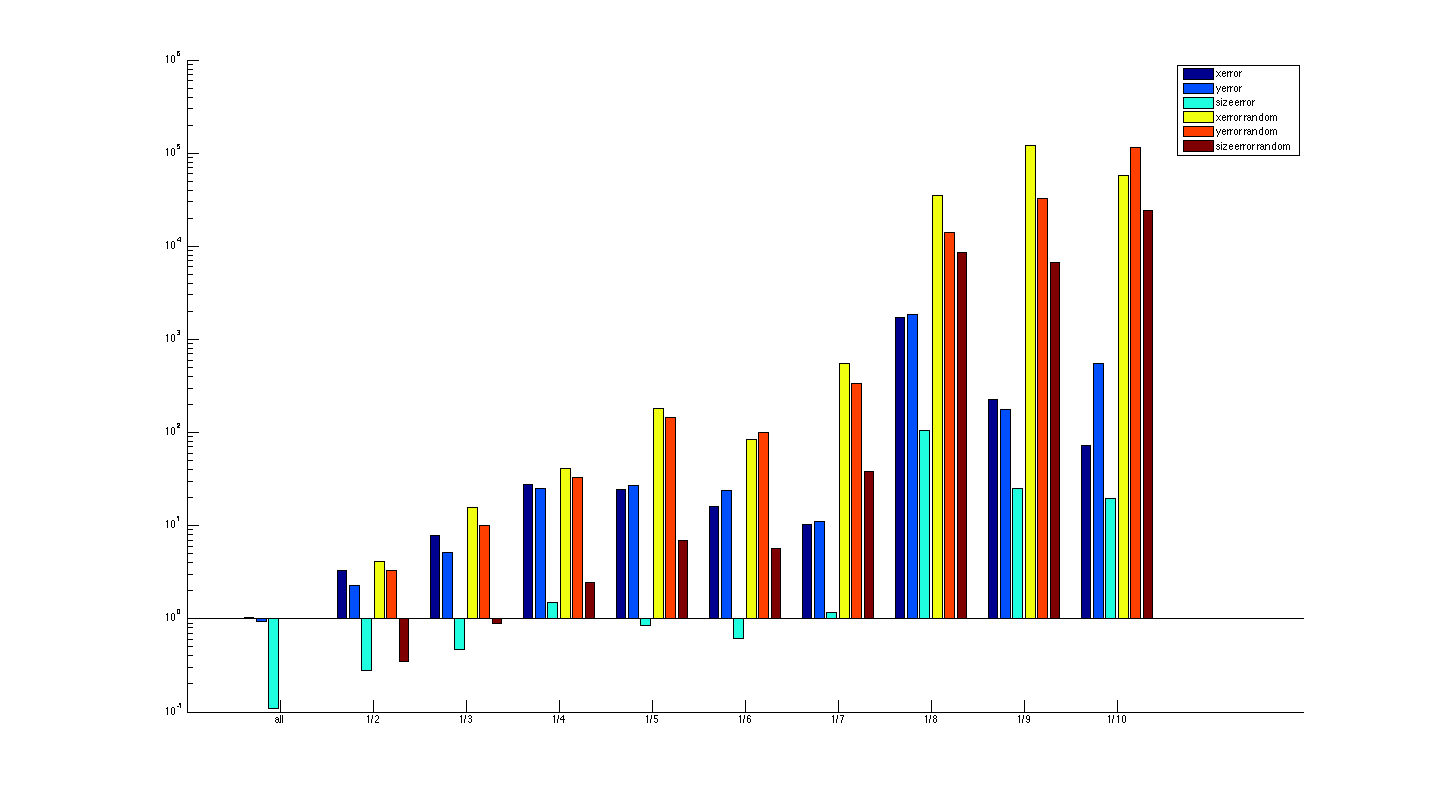
\includegraphics[width=.5\textwidth]{kalman_nov_1.png}
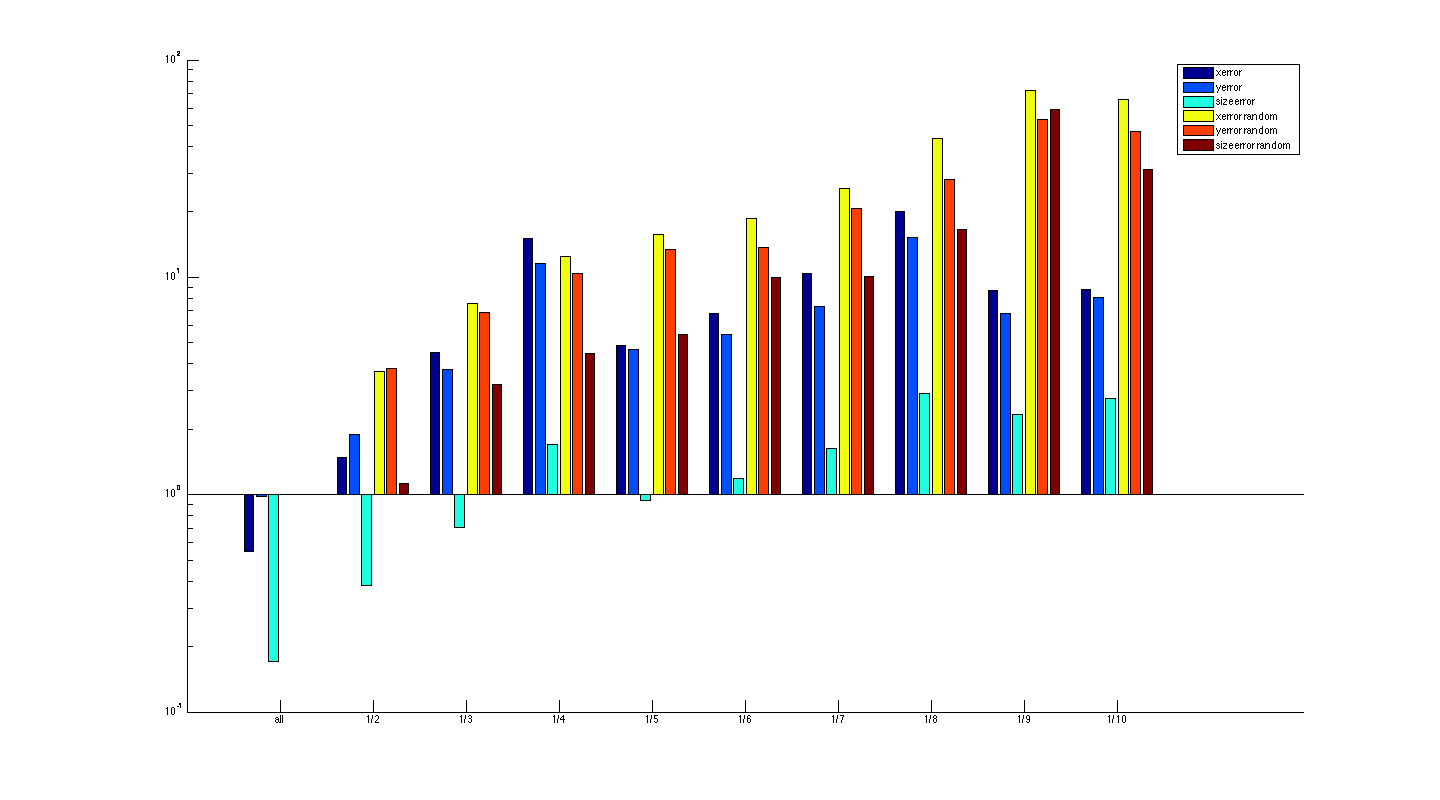
\includegraphics[width=.5\textwidth]{kalman_nov_2.png}
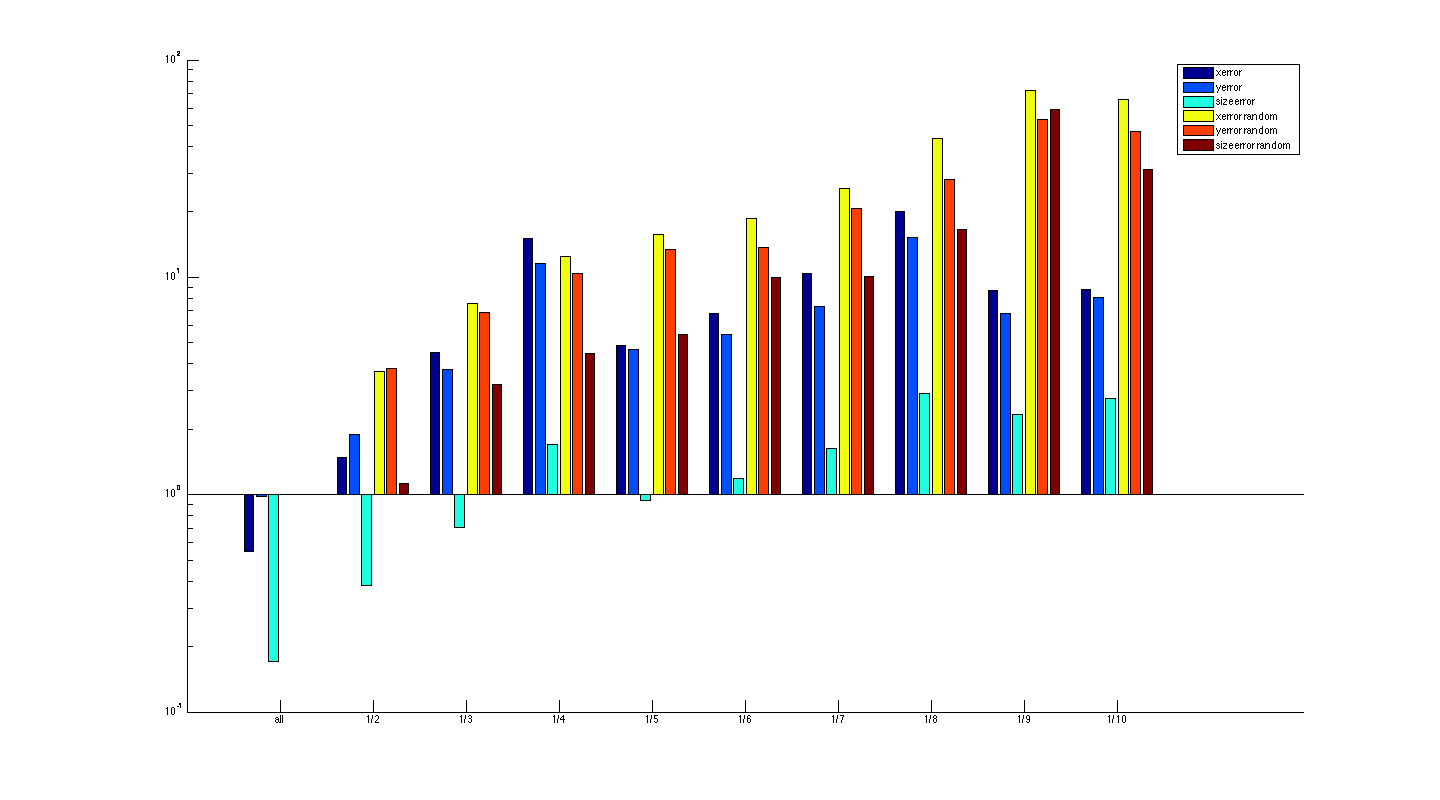
\includegraphics[width=.5\textwidth]{kalman_nov_2.png}
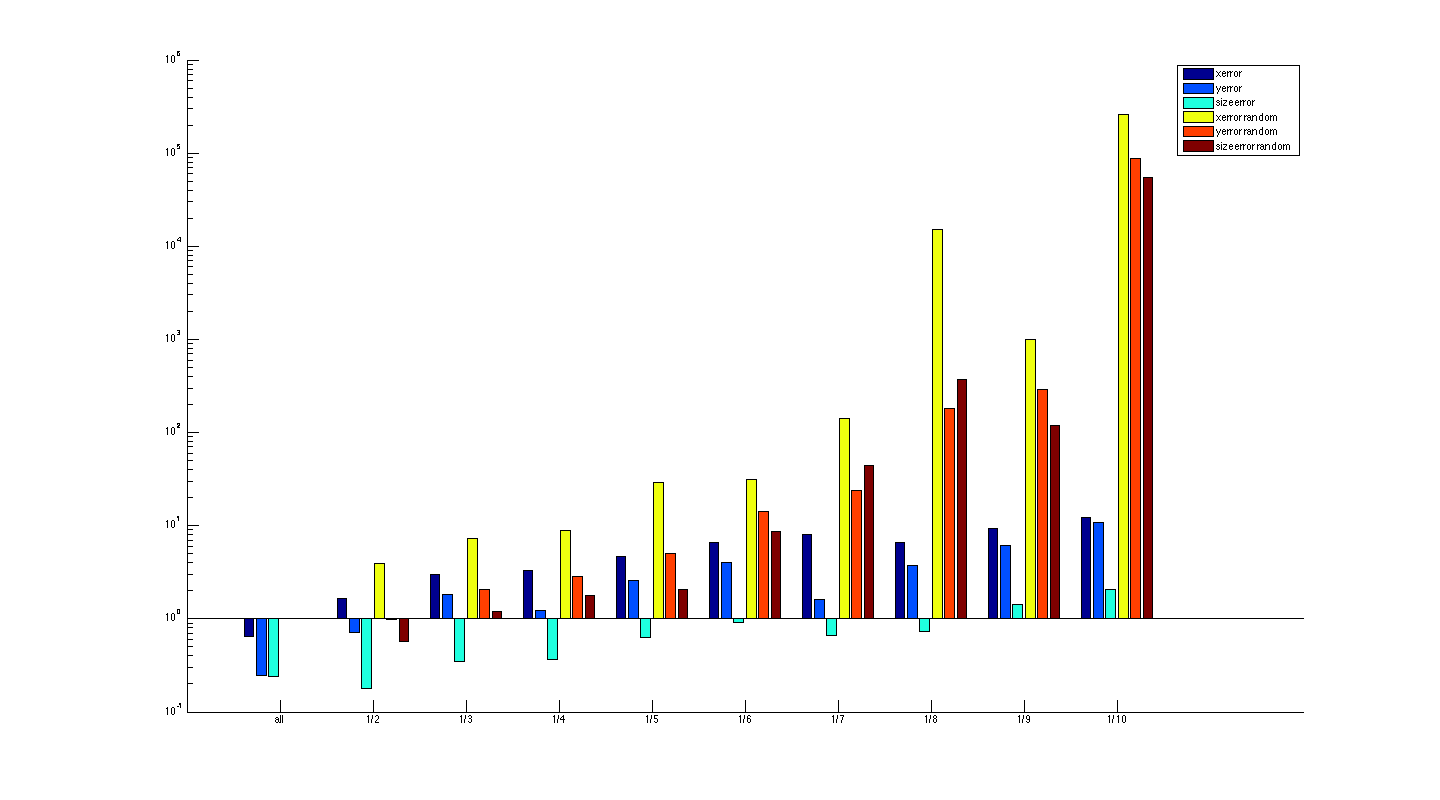
\includegraphics[width=.5\textwidth]{kalman_dec_1.png}
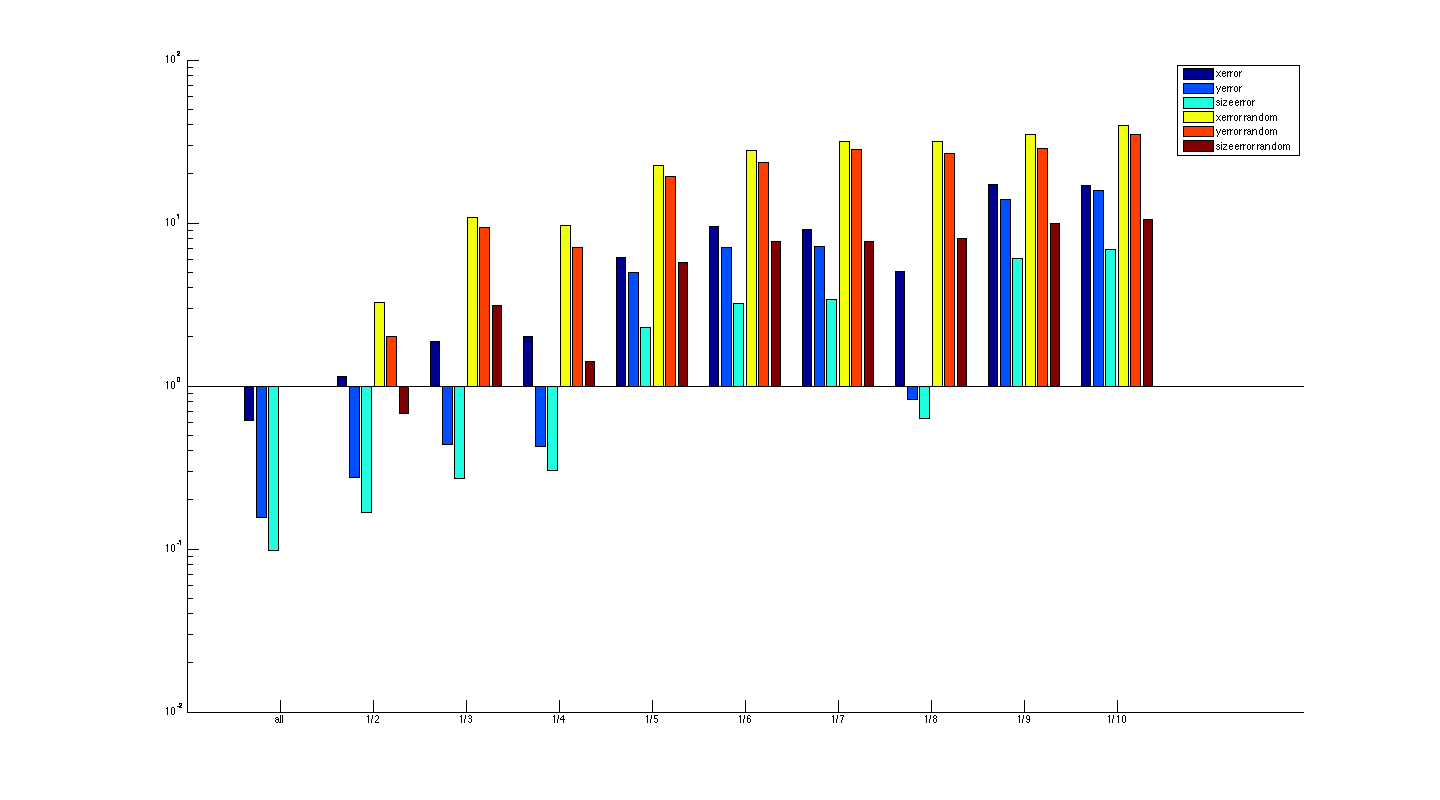
\includegraphics[width=.5\textwidth]{kalman_dec_2.png}
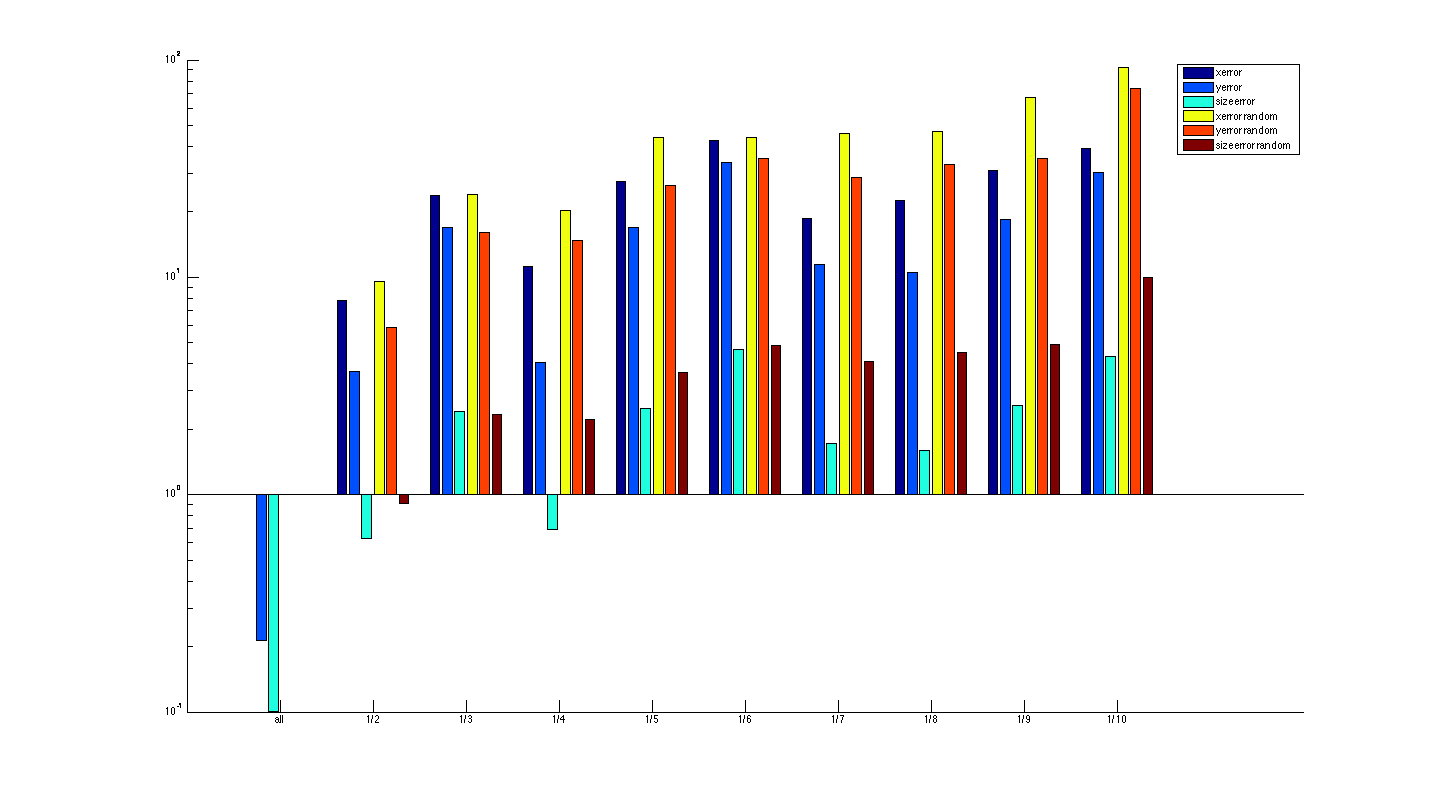
\includegraphics[width=.5\textwidth]{kalman_dec_3.png}
\caption{Kalman filter error on all datasets.  It is important to note that the Kalman filter on equally spaced sampling produces results which are often acceptable as compared to  random sampling. This implies that systems which evaluate detections at a subset of frames could be designed.}
\label{fig:kalman_error}
\end{figure}


When we combined the Kalman filter with the local homography estimation for tracking the fiducial marker we get a prediction of the corners of the tag for every frame.  We compare the corners predicted with the ground truth corners defined by the April tag detections.  We report results on no subsampling, 1/2, 1/5, and 1/10th both random and equally spaced.  When we have a detection in the subsampled data we restart the tag at the ground truth location, as such for the even sampling we see that there is a cyclic response of drift for the sampling period and then a correction.  Random sampling has occassional bad periods where there is no correction phase for a long period and the result becomes quite bad.
\begin{figure}
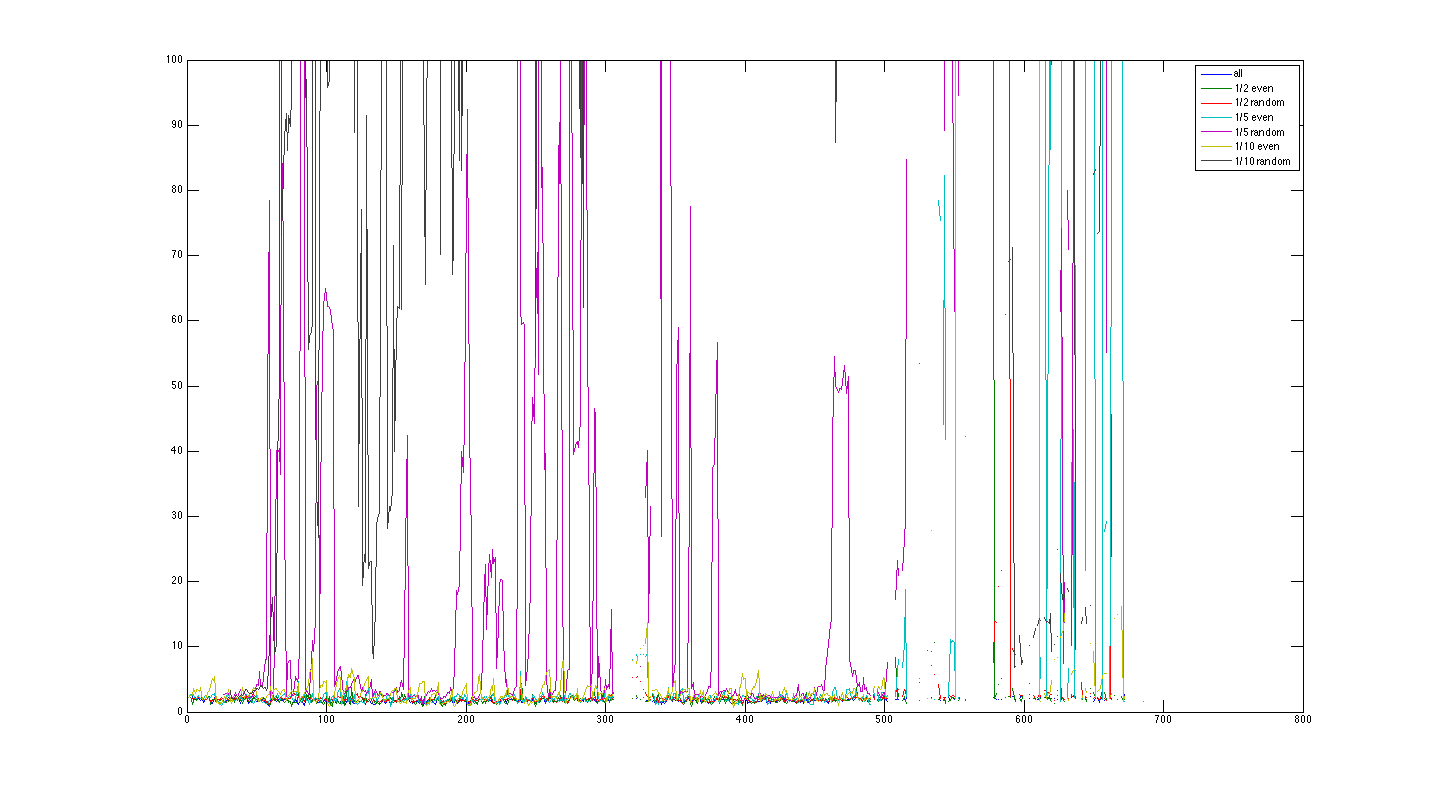
\includegraphics[width=.5\textwidth]{Corner_error_nov1.png}
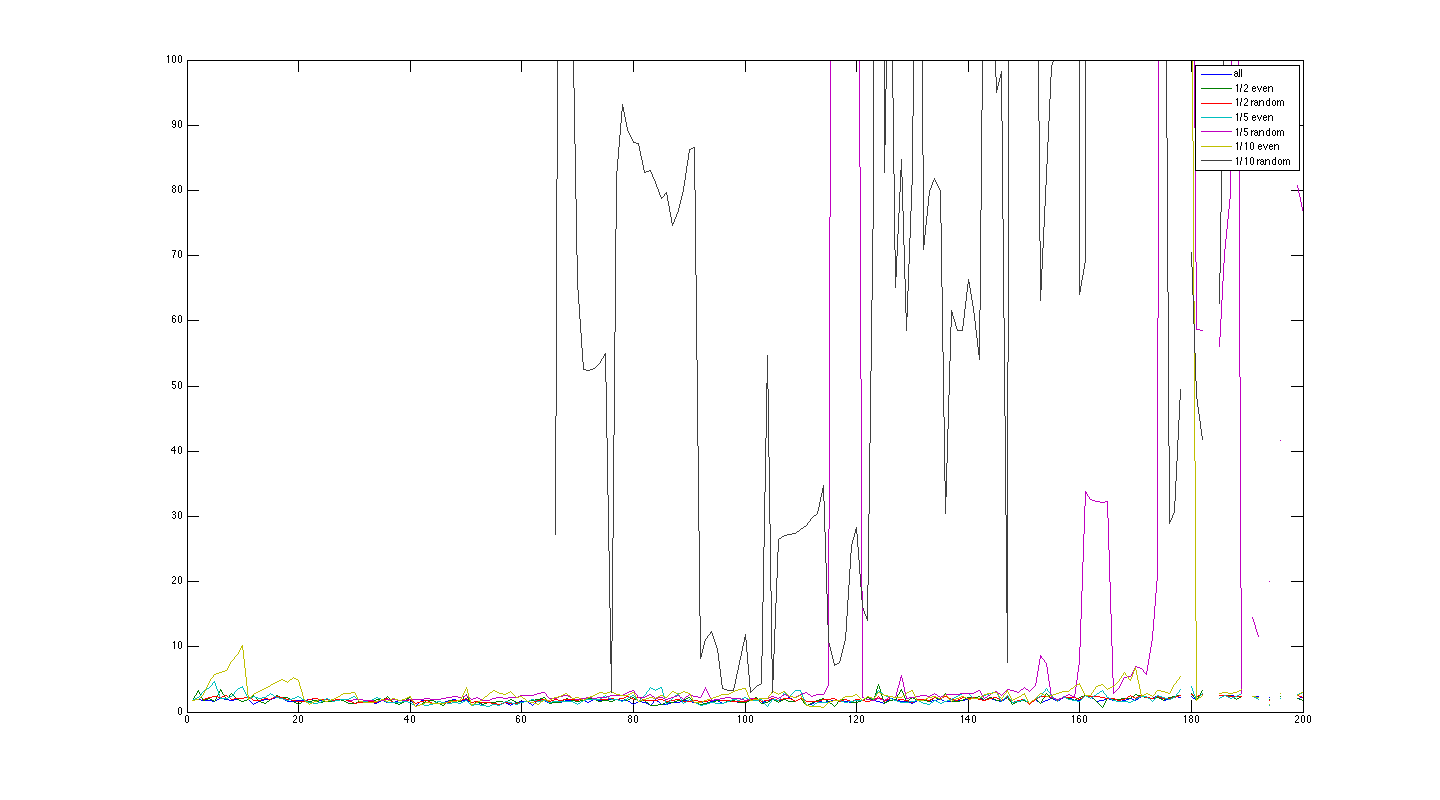
\includegraphics[width=.5\textwidth]{Corner_error_nov2.png}
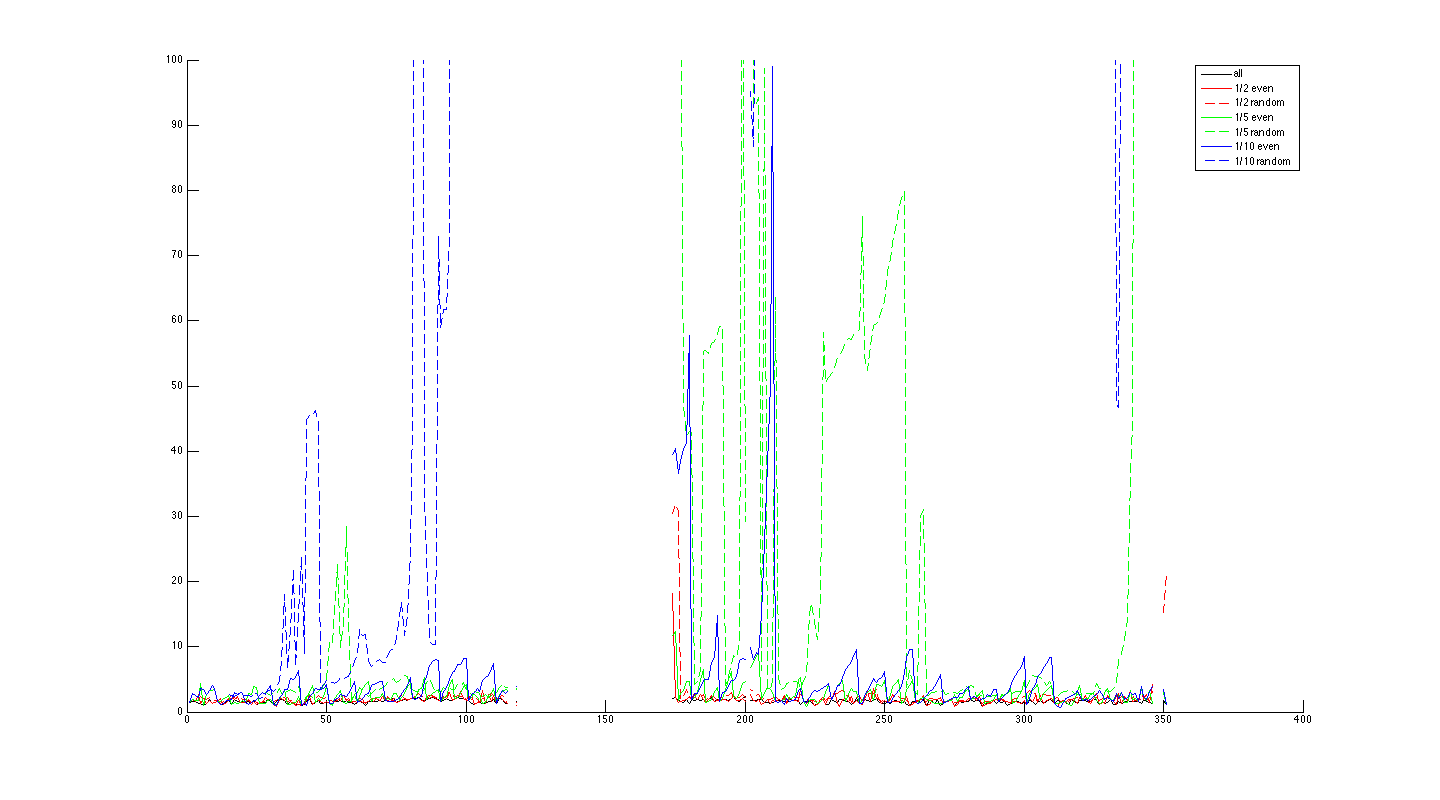
\includegraphics[width=.5\textwidth]{Corner_error_nov3.png}
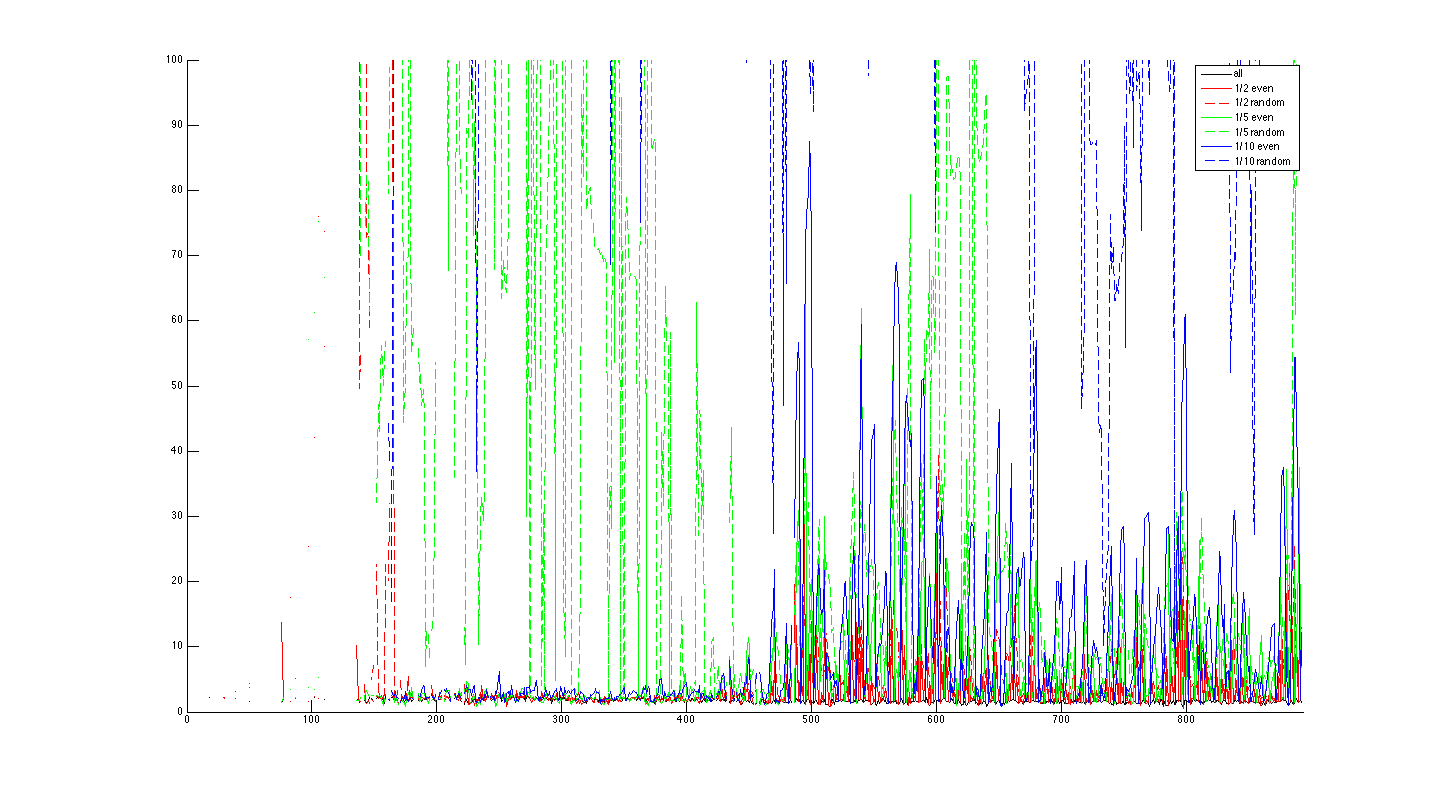
\includegraphics[width=.5\textwidth]{Corner_error_dec1.png}
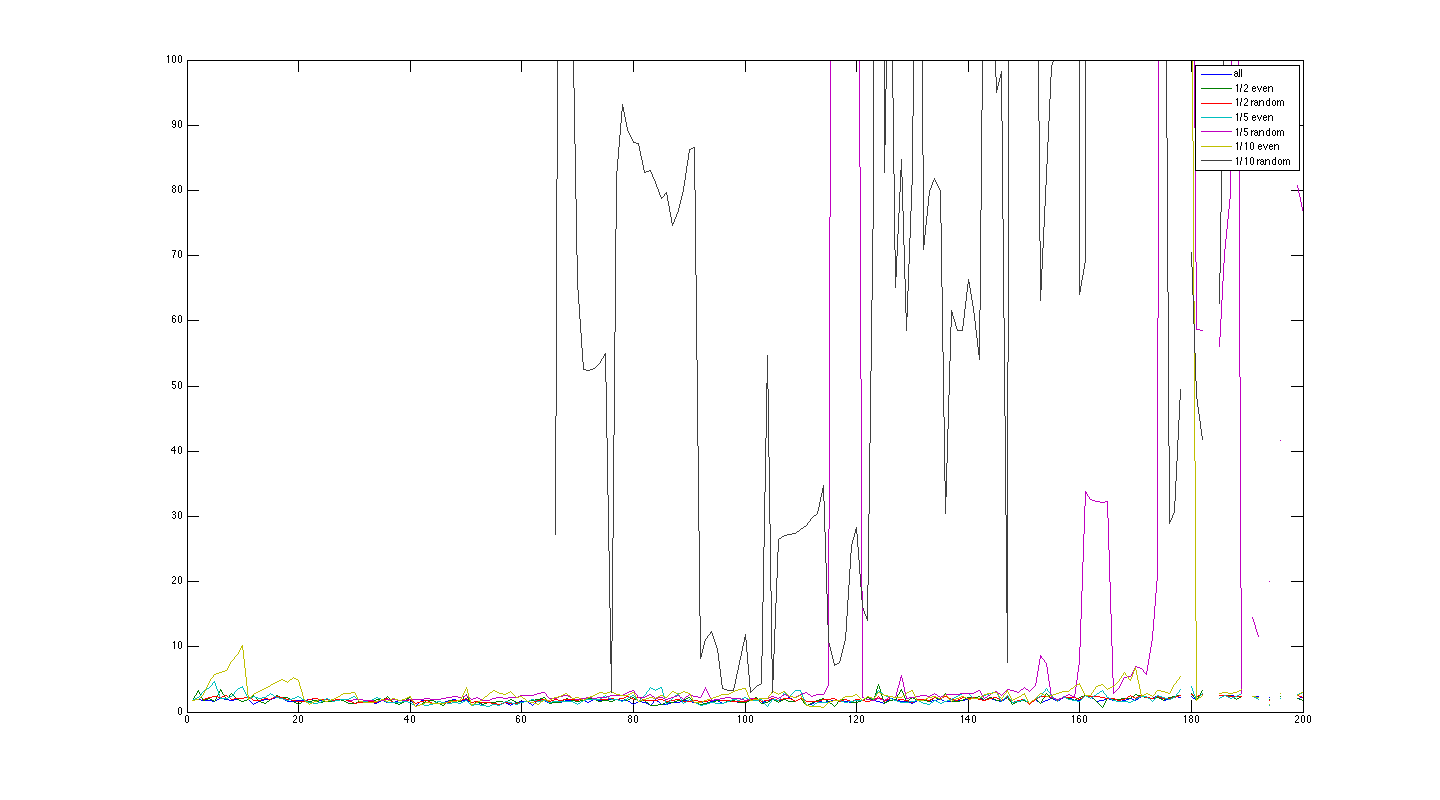
\includegraphics[width=.5\textwidth]{Corner_error_nov2.png}
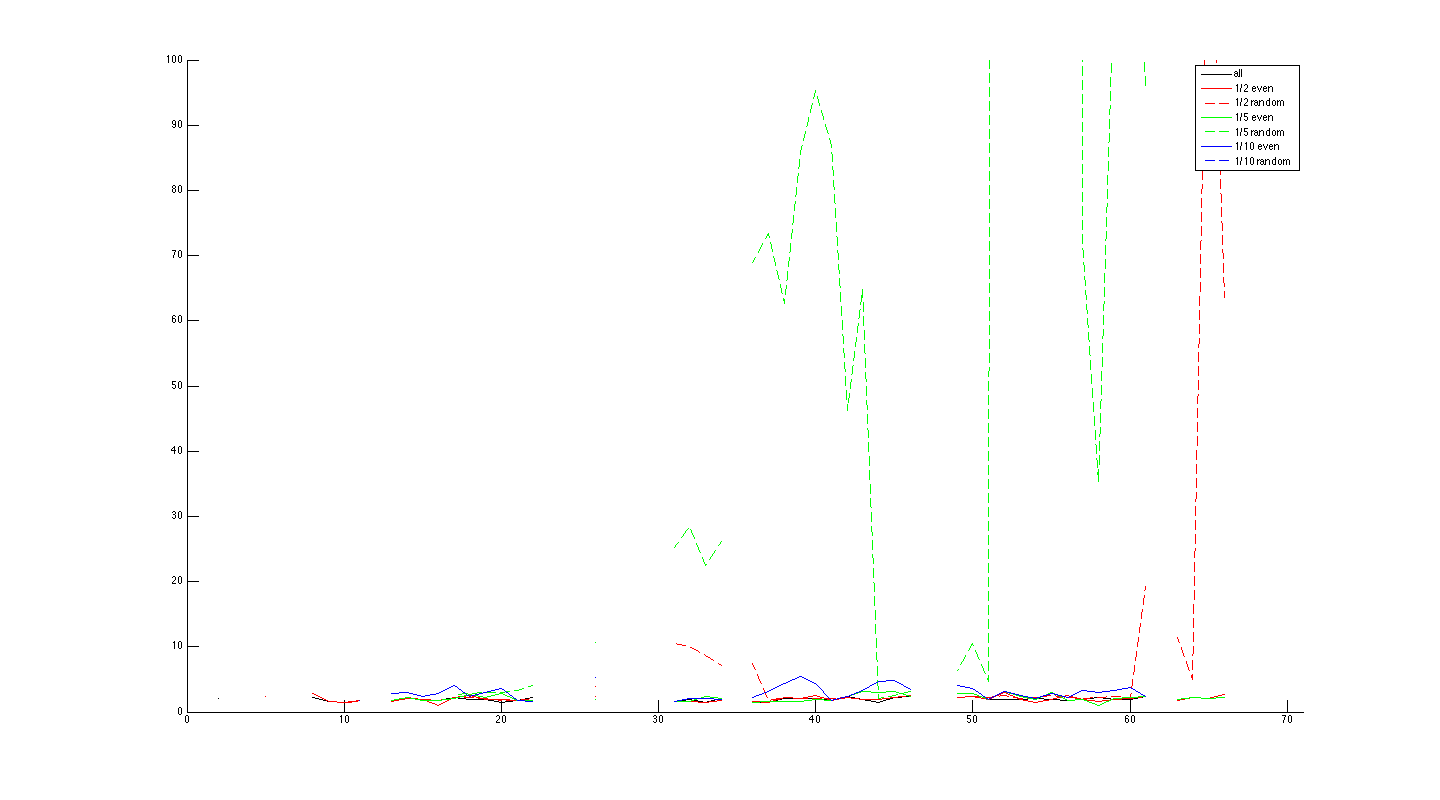
\includegraphics[width=.5\textwidth]{Corner_error_dec3.png}
\caption{Error of the corners of the fiducial marker predicted by our system with respect to the ground truth April Tag detector.  Blank areas represent locations where the April Tag was not detected by the ground truth detector.  See our later experiment for the analysis of our detector in these areas.}
\label{fig:corner_error}

\subsection{Datasets}



\end{document}
